% From assignment:
% Prioritize measurements and analysis/interpretation!

% Demonstrate use of tools (profiling, ...) , and simple performance
% model.

\subsection{Compilation flags}

For the improved OpenMP, we continued with investigating the
performance effect of compilation flags. For an R package the \texttt{CXX}
flags can be set in multiple ways, we first tried to change the
R package specific setting, in \texttt{/src/Makevars}, but for our
settings to achieve precedence over the Ferlin system settings we had
to set the flags in \texttt{.R/Makevars}. In Figure
\ref{fig:flagScaling} we compare the performance effect of using
the compilation flags \texttt{-O2}, \texttt{-O3} and \texttt{-Ofast
  -funroll-all-loops} for a number of cores. The effect of setting
compilation flags is small in comparison to the effect of using
multiple cores.

\begin{figure}[!htbp] \centering
  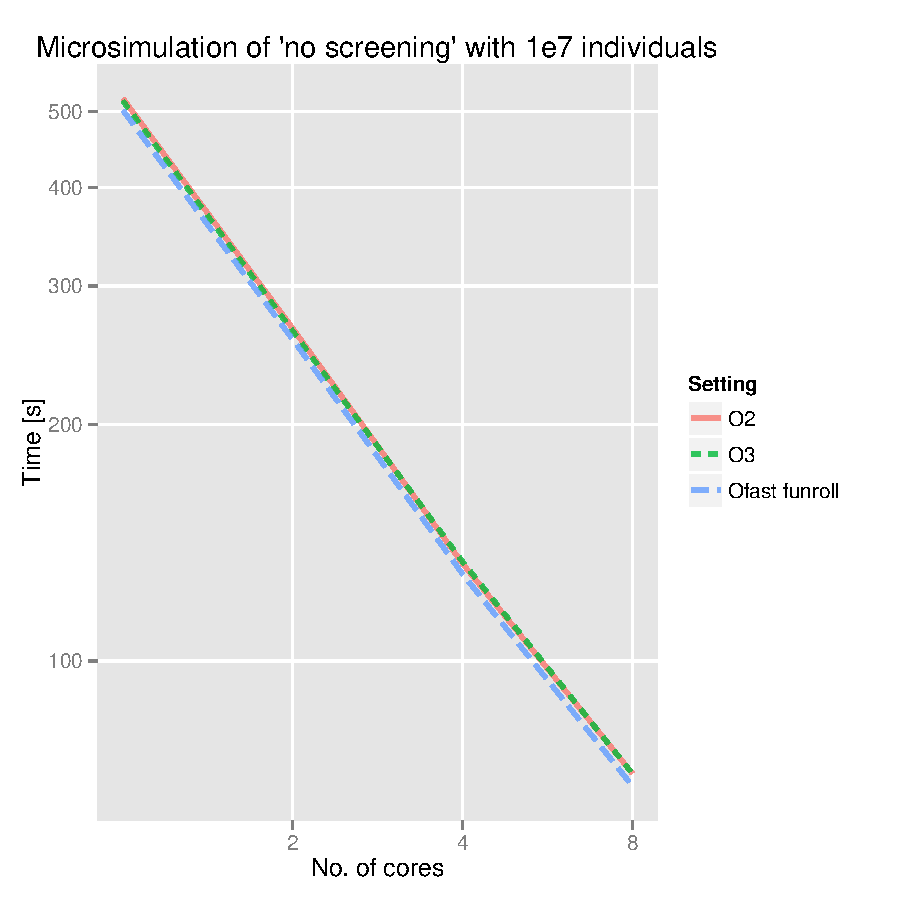
\includegraphics[height=0.5\textheight]{images/flagsProfiling.pdf}
  \caption{Performance effect of using the compilation flags \texttt{-O2}, \texttt{-O3} and \texttt{-Ofast -funroll-all-loops} for a number of cores}
  \label{fig:flagScaling}
\end{figure}


\subsection{Hybrid openMP and MPI}



%%% Local Variables: 
%%% mode: latex 
%%% TeX-master: "report" 
%%% End:
